\documentclass{beamer}
\usepackage{amsmath,amssymb}
\usepackage{graphicx}
\usepackage{siunitx}
\sisetup{per-mode=symbol}
\usepackage{gvv}
\usepackage{listings}
\usepackage{xcolor}

% Code style
\lstset{
  basicstyle=\ttfamily\scriptsize,
  breaklines=true,
  frame=single,
  numbers=left,
  numberstyle=\tiny,
  keywordstyle=\color{blue},
  commentstyle=\color{green!50!black},
  stringstyle=\color{red!60!black},
  showstringspaces=false
}

\title{4.12.20}
\author{ai25btech11015 -- M Sai Rithik}
\date{}

\begin{document}
\frame{\titlepage}

\begin{frame}
\frametitle{Question}
One vertex of the equilateral triangle with centroid at the origin and one side as
\[
x + y - 2 = 0
\]
is
\[
\text{(a) }(-1,-1) \quad 
\text{(b) }(2,2) \quad 
\text{(c) }(-2,-2) \quad 
\text{(d) }(2,-2).
\]
\end{frame}

\begin{frame}
\frametitle{Step 1: Condition for centroid}
Let the vertices be
\[
\Vec{A},\; \Vec{B},\; \Vec{C}.
\]
Since centroid is at origin,
\begin{equation}
\Vec{A} + \Vec{B} + \Vec{C} = \Vec{0}.
\label{eq:centroid}
\end{equation}
\end{frame}

\begin{frame}
\frametitle{Step 2: Side equation}
Suppose side \(BC\) lies on the line
\begin{equation}
x + y - 2 = 0,
\label{eq:line}
\end{equation}
i.e.,
\[
\myvec{1 & 1}\Vec{x} = 2.
\]
Normal vector:
\[
\Vec{n} = \myvec{1 \\ 1}, \quad
\Vec{m} = \myvec{1 \\ -1}.
\]
\end{frame}

\begin{frame}
\frametitle{Step 3: Alternative choice of side}
If \(AB\) lies on line \eqref{eq:line}, then \(C\) lies on perpendicular from origin:  
\[
\Vec{x} = t\myvec{1 \\ -1}.
\]

Check options: only \((2,-2)\) satisfies this condition.  
\end{frame}

\begin{frame}
\frametitle{Final Answer}
The required vertex is
\[
\boxed{(2,-2)}
\]

\begin{figure}[h!]
    \centering
    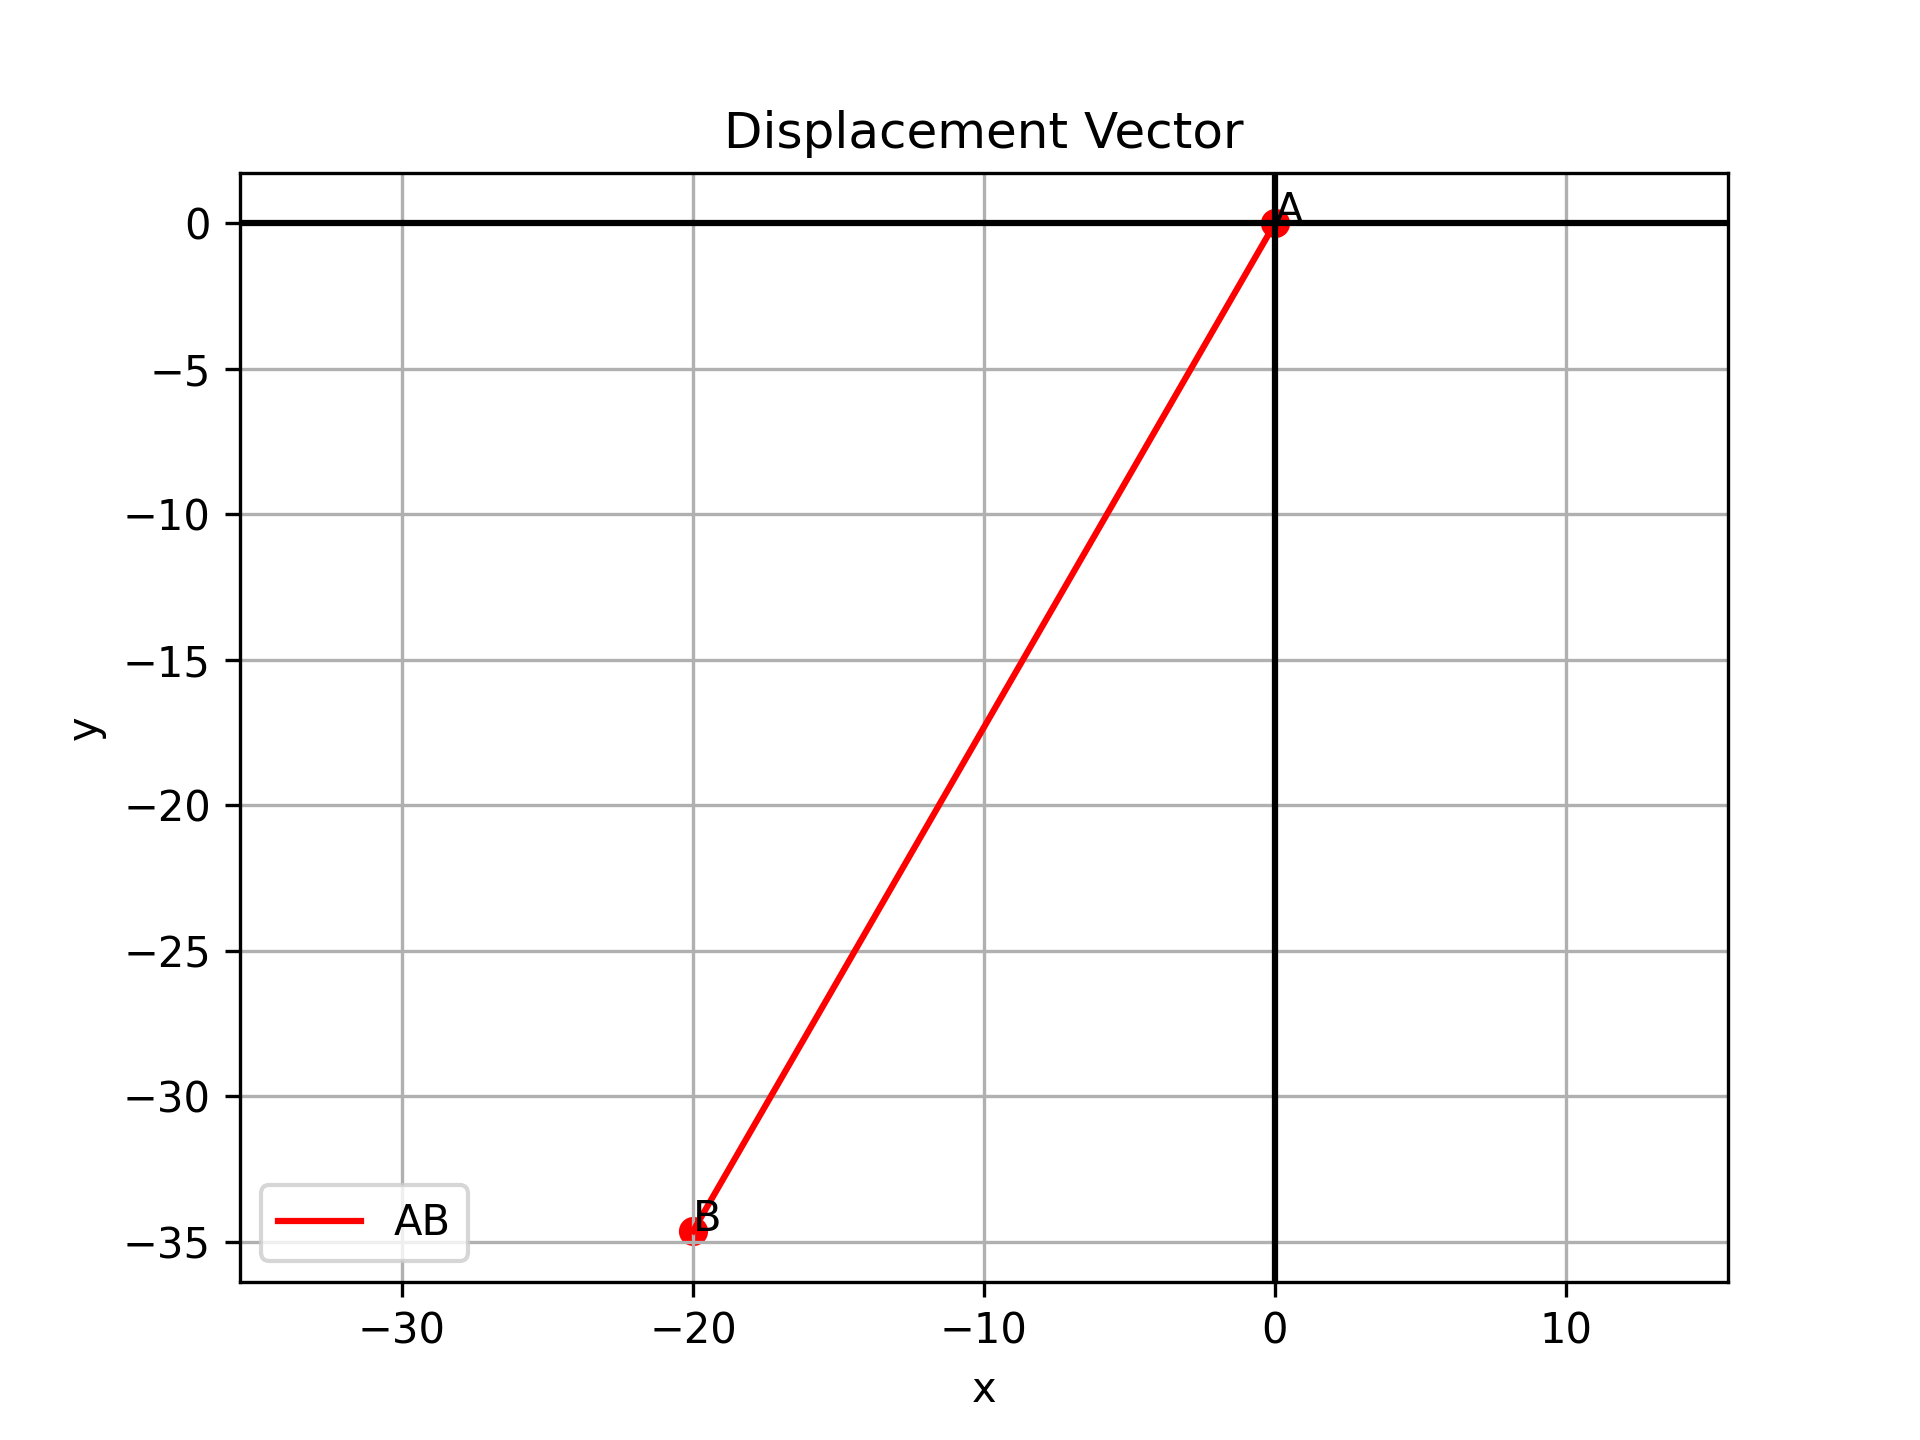
\includegraphics[width=0.6\linewidth]{figs/fig.png}
    \caption{Equilateral triangle with centroid at origin and one side on $x+y-2=0$.}
\end{figure}
\end{frame}


\end{document}
